\chapter{Object detection and segmentation}
In this thesis we focus on tracking objects in video data using target tracking algorithms with dynamic detection probability due to the existence of obstacles that cause sensors to not detect objects in certain situations. But first, we need to have a sensor for detecting objects in a
frame.


\section{Object detection}
Object detection is a fundamental task in computer vision that involves identifying and localizing objects
within images or video frames, respectively. Unlike image classification, which assigns a single label to an entire
image, object
detection algorithms aim to detect multiple objects of various classes and localize them with bounding boxes.
Alongside image classification and object detections, there are other tasks, such as semantic segmentation and
instance segmentation. Figure \ref{fig:seg_type} shows differences between these types of image processing tasks.

\begin{figure}
  \centering
  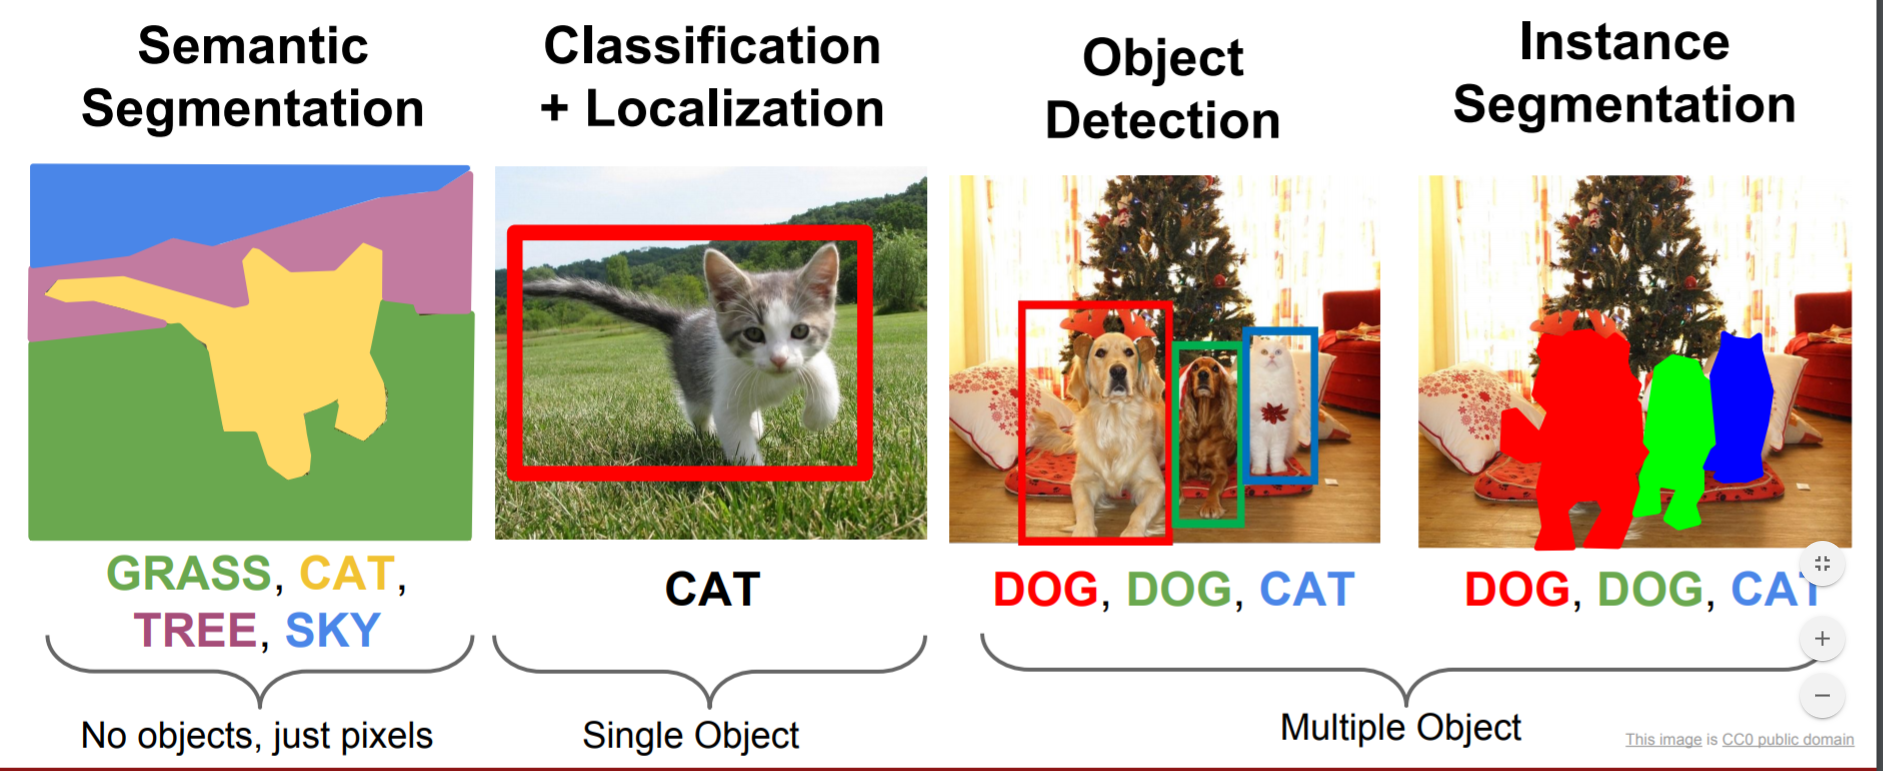
\includegraphics[width=\linewidth]{text/chapter_03/imgs/segmentation-types}
  \caption{Image detection and segmentation task types. (Source: \href{https://techvidvan.com/tutorials/image-segmentation-machine-learning/}{techvidvan.com}.)}
  \label{fig:seg_type}
\end{figure}

The development of object detection algorithms has evolved significantly over the years, driven by advances in deep
learning, dataset availability and computational power. Traditional object detection methods relied on handcrafted
features and machine learning algorithms, such as sliding window-based classifiers, histogram of oriented gradients (HOG) \cite{HoOGDalal2005}, and Haar cascades \cite{HaarCascadesLi2016}. While effective in certain scenarios, these methods often lacked robustness and scalability, particularly in complex and cluttered scenes.

With the advent of deep learning, convolutional neural networks (CNNs) improved the field of object detection. CNNs are
capable of automatically learning hierarchical representations of data, making them well suited for image analysis
tasks. The rise of CNN-based approaches has led to significant improvements in object detection accuracy and efficiency.
At its core, a convolutional neural network is comprised of multiple layers, each designed to perform specific operations on input data, typically images. The fundamental layers in a CNN include convolutional layers, pooling layers, and fully connected layers.
\begin{enumerate}
  \item \textbf{Convolutional layers:} These layers are responsible for extracting features from the input data. They consist of filters (also called kernels) that slide across the input image, performing a mathematical operation known as convolution. Each filter detects certain patterns or features, such as edges, textures, or shapes. By convolving the filters with the input image, the CNN can capture hierarchical representations of features, starting from simple edges and gradients to more complex structures.
  \item \textbf{Pooling layers:} Pooling layers are interspersed between convolutional layers to reduce the spatial dimensions of the feature maps while retaining important information. Common pooling operations include max pooling and average pooling, which downsample the feature maps by taking the maximum or average value within each pooling region. This downsampling helps in reducing computational complexity and controlling overfitting by enforcing spatial invariance.
  \item \textbf{Fully connected layers:} These layers are typically placed at the end of the CNN and serve to classify the features extracted by the convolutional layers. Each neuron in a fully connected layer is connected to every activation in the previous layer, forming a dense network. These layers use techniques like softmax activation to produce probability distributions over the classes in a classification task or regression outputs in a regression task.
\end{enumerate}
It is important to note, that it is common to combine more convolutional, pooling and fully connected layers with differently sized kernels in the architecture to improve the performance. Example of such architecture is shown in Figure \ref{fig:CNNArchitecture}
\begin{figure}
  \centering
  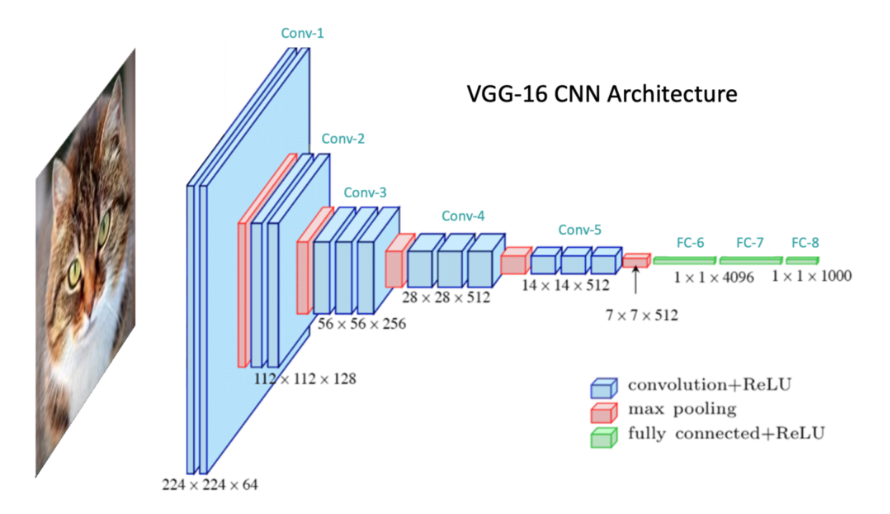
\includegraphics[width=\linewidth]{text/chapter_03/imgs/CNN}
  \caption{CNN architecture example. (Source \href{https://learnopencv.com/understanding-convolutional-neural-networks-cnn/}{learnopencv.com})}
  \label{fig:CNNArchitecture}
\end{figure}
During training, CNNs use a process called backpropagation to adjust the parameters (weights and biases) of the network based on the disparity between the predicted outputs and the ground truth labels. This optimization process aims to minimize a predefined loss function, such as cross-entropy loss for classification tasks or mean squared error for regression tasks. By iteratively updating the parameters using optimization algorithms like stochastic gradient descent (SGD) or its variants, CNNs gradually learn to recognize and classify patterns within the input data, ultimately improving their performance on various visual tasks such as object detection and segmentation.


Object detection poses several challenges, including variations in object appearance, scale, orientation, occlusion, and cluttered backgrounds. Additionally, real-world images often contain multiple objects of different classes, making it essential for detection algorithms to handle overlapping and partially visible objects.

Furthermore, object detection systems often have to balance accuracy and speed to meet the demands of real-time
applications. Achieving high detection accuracy while maintaining fast inference times is a fundamental challenge,
especially for devices with low hardware resources and applications requiring low-latency processing.

Object detection algorithms typically consist of several components:

\begin{itemize}
  \item \textbf{Input processing:} Images or video frames are preprocessed to standardize their format and size, often
involving resizing, normalization, and data augmentation to enhance model generalization.
  \item \textbf{Feature extraction:} Feature extraction is performed to capture relevant information from the input
  data. In deep learning-based approaches, convolutional neural networks are commonly used to extract hierarchical features that encode object appearance and spatial relationships.
  \item \textbf{Localization:} Localization involves predicting the spatial extent of objects within the image using
bounding boxes. This step requires regression or classification to estimate bounding box coordinates and confidence scores for object presence.
  \item \textbf{Classification:} Object classification assigns class labels to detected objects based on their visual
  appearance. Classification models are trained to distinguish between different object categories, enabling accurate identification of objects within the scene.
  \item \textbf{Post-processing:} Post-processing techniques, such as non-maximum suppression (NMS), are applied to
  refine detection results, suppress duplicate detections, and improve localization accuracy.
\end{itemize}



  \subsection{YOLO}

In the realm of object detection, the emergence of You Only Look Once (YOLO) represents a paradigm shift, propelled by the fusion of deep learning and innovative architectural design. YOLO stands as a testament to the transformative power of convolutional neural networks (CNNs) in redefining the landscape of computer vision applications, particularly in real-time object detection scenarios. This object detector was proposed by Developed by Joseph Redmon, Santosh Divvala, Ross Girshick, and Ali Farhadi in \cite{YOLORedmon2016}.

At its core, YOLO introduces a groundbreaking concept: the ability to predict bounding boxes and class probabilities for objects within an image in a single pass through the neural network. This departure from traditional object detection methods, which often involve multi-stage processes and post-processing steps, marks a significant leap forward in efficiency and speed. By consolidating object localization and classification into a unified framework, YOLO streamlines the detection pipeline, enabling seamless integration into various applications requiring rapid decision-making based on visual data.


A distinguishing feature of YOLO lies in its holistic approach to image analysis. Unlike conventional methods that segment images into regions of interest for further processing, YOLO takes a global perspective by dividing the input image into a grid and processing it as a whole. This global context consideration not only enhances the model's understanding of spatial relationships but also reduces the risk of misclassification, particularly in complex scenes with multiple objects. Each bounding box prediction includes coordinates $(x, y)$ for the center of the box, width, height, and confidence score indicating the likelihood of containing an object. Additionally, class probabilities are estimated for each bounding box to determine the object category. YOLO employs a loss function that penalizes localization errors, confidence errors, and classification errors.
This loss function is optimized during training using labeled datasets to learn accurate object representations. Moreover, YOLO adopts anchor boxes to improve localization accuracy and handle scale variations of objects within the image.

The evolution of YOLO over successive versions underscores its adaptability to diverse use cases and computational environments. While early iterations prioritized speed, subsequent iterations like YOLOv4 and YOLOv5 have aimed to enhance accuracy without compromising real-time performance \cite{YoloVersions2022}. This flexibility in model selection empowers users to tailor YOLO to their specific requirements, whether it be for surveillance systems demanding rapid detection or autonomous vehicles requiring precise object localization.

Compared to traditional object detection methodologies such as region-based convolutional neural networks (R-CNN) \cite{MaskRCNN2017} and single-shot detectors (SSD), YOLO stands out for its simplicity and efficiency. By eliminating the need for complex post-processing steps and leveraging a unified architecture for object detection (see Figure \ref{fig:yoloArchitecture} for YOLO architecture), YOLO achieves a fine balance between speed and accuracy. This versatility extends YOLO's applicability across a myriad of domains, including but not limited to autonomous driving, industrial automation, healthcare imaging, and augmented reality.

\begin{figure}
  \centering
  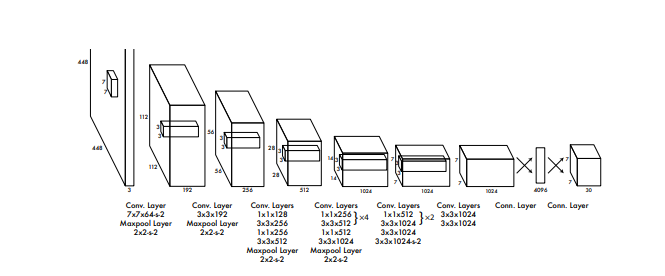
\includegraphics[width=\linewidth]{text/chapter_03/imgs/YOLO_architecture}
  \caption{Yolo architecture proposed in \cite{YOLORedmon2016} has 24 convolutinal layers followed by 2 fully connected layers. Convolutional layers were pretrained on the ImageNet classificator at half resolution (224 x 224 input image) and the doubled the resolution for detection. (Source \cite{YOLORedmon2016}.)}
  \label{fig:yoloArchitecture}
\end{figure}


\section{Object segmentation}
\cite{IBM}
Object segmentation involves partitioning an image into semantically meaningful regions and associating each region
with a specific object instance. Unlike object detection, which identifies objects at the bounding box level, segmentation provides pixel-level delineation of object boundaries. This fine-grained information is invaluable for tasks such as image understanding, scene understanding and image manipulation.

Semantic segmentation assigns a class label to each pixel in the image, effectively partitioning the image into regions corresponding to different object categories. Fully Convolutional Networks (FCNs) and their variants, such as U-Net and DeepLab, have demonstrated remarkable success in semantic segmentation tasks by leveraging the power of convolutional neural networks for dense pixel-wise predictions \cite{SemanticSegmentationGuo2022}.

Instance segmentation, on the other hand, extends semantic segmentation by distinguishing between individual object instances of the same class. This task requires not only segmenting objects but also differentiating between instances of the same class, even if they overlap or occlude each other. Mask R-CNN, an extension of Faster R-CNN, combines region-based object detection with instance segmentation, achieving state-of-the-art results in both tasks.

Despite significant advancements, object detection and segmentation still face several challenges. These include handling scale variations, occlusions, cluttered backgrounds, and fine-grained object attributes. Additionally, achieving real-time performance while maintaining high accuracy remains a critical goal for many applications.

  \subsection{Segment anything}